\documentclass[a4paper,10pt]{article}
\usepackage{src/preamble}

\usepackage{biblatex}
\addbibresource{ResearchPaperBib.bib}

\begin{document}

\noindent
\begin{center}
	\textbf{{\Large DEPLOYMENT OF LLMs AT THE EDGE OF THE 6G NETWORK}} \\
\end{center}

\noindent
\textbf{Author: Alessandro Biagiotti} \hfill \textit{Università degli studi di Milano, Milano, Italia}
\\

\noindent
\textbf{ABSTRACT:}
\\
LLMs are definitely the most interesting discovery of this century, they have been deployed in many different fields and have proven themselves worthy in many different situations. Currently, research for the next Mobile communication standard has started and the idea of pushing LLMs close to the end users has stimulated the interest of many researchers.

In this paper I will explore the opportunities and the difficulties of deploying LLMs at the edge of the 6G network as well as providing some brief insights on solutions that caught the attention of the scientific community.

\bigskip
\noindent
\textbf{KEYWORDS:}
\\
\textit{6G, AI, LLM, paper-reviewing}

\clearpage

\noindent
\textbf{INTRODUCTION:}
\label{sec:introduction}
\\
\externaldocument{../main}

The impressive development of AI technologies that followed the publication of the notorious article
"Attention is all you need"\cite{attention} has pushed research teams to try and incorporate LLMs
and other such models into every aspect of human life. From consumer electronics to cars, aerospace
and industrial applications AI is going to be a pervasive part of society from now on.

Every ten years the mobile communication standard changes and a new iteration is released, 2020
paved the way to 5G era, and now the research and development process has begun for the next mobile communication standard.
As stated in \cite{6ainets}, 6G is "poised to revolutionize the landscape by delivering
unprecedented speed, reliability and security". This is a big promise, users will not be facing the
next incremental improvement that they are so used to seeing nowadays with consumer electronics,
a revolutionary way of interacting with the network is apparently waiting for us less than ten years
from now.

6G is in fact meant to marry Wireless Networks and AI creating a chimera capable of speed,
customization and pervasiveness. This new standard is meant to bring to life an infrastructure that
will be able to support the immense requirements of the upcoming field of IoT.

\bigskip

All of this sounds incredibly promising on paper but, as it is known, big changes need to overcome even
bigger challenges: How can one put AI in the hands of the users and make it work reliably? How can
one make sure that LLMs behave correctly and reply in a timely fashion? How can one
assure that the network is functioning correctly and the model is correctly trained? How can we
handle the ever pressing problem of data security?

These are just some of the questions that one could be asking about 6G research. Due to the sheer size of the topic, for this
paper I chose to delve into some paper reviewing alongside some considerations about the specific
topic of Artificial Intelligence integration with the network, in particular in the next sections I
will go through: \ref{sec:ai-agents} in which I will be giving a very brief
overview of the 6G network and then move on to explaining what types
of AI agents are being used in the field of Wireless networks research, \ref{sec:opportunities} in
which I will be introducing the different opportunities that AI brings to the table, and I will
give some pointers as to what components are essential in the 6G architecture, \ref{sec:technical-limitations} in this section I will be explaining which are the biggest technical limitations for the implementation of LLMs at the edge of wireless networks, furthermore I will go through some solutions that have been provided to the above problems; in the last section \ref{sec:future-challenges} I will dedicate myself to drawing some
conclusions and pointing at some research topics that might be of active interest.

\clearpage

\noindent
\textbf{6G OVERVIEW AND AI AGENTS:}
\phantomsection
\makeatletter\def\@currentlabel{\texttt{(I)}}\makeatother
\label{sec:ai-agents}
\\
\externaldocument{../main.tex}

Mobile communication technologies have been a standard evolving since the very first
generation of the technology released in 1981. Every ten years a new standard is formulated and
developed to propel the industry forward, the generational improvements were not necessarily
paradigm shifts, as an example, the move from 3G to 4G was more along the line of a performance bump,
meanwhile the passage to 5G and 6G represented and will represent a big leap forward in terms of
what the network is able to support and what will be able to bring to the table in the future.

At the moment researchers in all the fields are trying to find the limits of the new standard to
push it even further and also to make 6G achievable on a very large scale, we should expect the
first real world tests with end users in 2030. According to Nokia\cite{nokiabell} the six key aspects of the future generation of mobile communication technologies can be summarized in the following subsections.

\bigskip
\noindent
NEW SPECTRUM TECHNOLOGIES:
\phantomsection
\label{ssec:spectrum-technologies}

The objective with 5G was achieving a big enhancement of the performance of the mobile communication
network in both upload and download, it was therefore necessary to provide mobile systems with a new
type of antenna that was able to work with millimeter waves (wavelength in the realm of the
millimeters), the available spectrum bands were:
\begin{itemize}
	\item 24 - 71 GHz which is high band 5G.
	\item 2.5 - 4.9 GHz which is the mid band 5G.
	\item 600 - 2600 MHz which is the low band 5G.
\end{itemize}
6G is thought to be implemented to use more wisely the space of millimeter waves and go beyond 71
GHz allowing for a higher spectral efficiency, the new standard will incorporate the 5G spectrum
standard, widen it, and take better advantage of the pre-existing bands. The structure of the spectrum is still being studied but the foundations seem to be the following:
\begin{itemize}
	\item 470 - 690 MHz extreme wide area coverage.
	\item 600 - 2600 MHz wide area coverage.
	\item 2.4 - 4.9 GHz urban capacity.
	\item 7 - 20 GHz extreme urban capacity.
	\item 24 - 71 GHz hotspot capacity.
	\item > 92 GHz will be the extremely short range communication system and is currently being
	      called the sub-TeraHertz band.
\end{itemize}

\bigskip
\noindent
AI AND MACHINE LEARNING:
\phantomsection
\label{ssec:ai-ml}

On the particular aspects of AI and Machine Learning we have many diverse weapons that can be put to
the service of the network or to the service of the users depending on the end goal that needs to
be achieved.

AI for the end user comes especially in the form of the so called LLM or Large Language Model. In
the last couple of years models like ChatGPT, GPT-4, LLaMa, etc... Have seen a spike not only in
their usage but also in the capabilities of the models that have been deployed. The multimodal
nature of some of the bigger models can be leveraged to allow a more reliable and detailed
resolution of the problems at hand and the use of prompt engineering techniques like "Chain of
Thought" and "Retrieval Augmented Generation" can turn the devices in the hand of end users into
powerful assistants that can handle many tasks both on-demand and autonomously.

Private automation, robotics and healthcare are just a couple of the fields that will be most
impacted by the addition of LLMs very close to the edge of the network. I'll go back at considering
the topic in the section \ref{sec:technical-limitations} to show how the feat that was just proposed
is extremely challenging and will require the employment of the most recent distributed machine
learning techniques to face it.

AI for the network is usually employed with the aim of trimming the resource usage allowing for a
more efficient employment of the available resources. This can be achieved using Reinforced learning models, or RLMs, these models should be
employed to help the network scale up and scale down whenever necessary to allow the usage of as
little resources as possible without hindering the quality of the offered services. Furthermore RLMs can be
used to help mitigate the problems that the employment of LLMs very close to the edge of the network
provoke.

\bigskip
\noindent
SECURITY AND TRUST:
\phantomsection
\label{ssec:security-trust}

The changes in the spectrum distribution of the network and the use of AI in the network forces
research to face a series of extremely important questions linked to private data security and
individual security.

Giving AI more power and control means that it's necessary to be able to
control its operation and make sure that is, not only, behaving according to specification, but also
not being fed polluted data during the training process by malicious third parties. Having extremely-high-frequency bands in the spectrum will expose communications to easy
eavesdropping, it's therefore necessary to create security procedures that allow communications to
remain private even when using these frequency bands.

\bigskip
\noindent
SENSING NETWORK:
\phantomsection
\label{ssec:sensing-network}

The use of Machine Learning and AI techniques coupled with a very high number of sensors will allow
the nodes of the network to sense the environment around them, this is an extremely useful technique to generate a Digital Twin of the real world, storing precious information about the surroundings and generating information through LLM inference.

Regarding the above Minrui Xu et al. \cite{pga} wrote a paper discussing how the multimodality of today’s LLMs alongside a wide array of sensors can be employed to generate automatically crash reports that can be further refined by seding them to a richer and more expressive LLM deployed at the edge of the network.

\bigskip
\noindent
EXTREME CONNECTIVITY:
\phantomsection
\label{ssec:extreme-connectivity}

The level of the services that are probably going to be brought to 6G require extremely fast and extremely
low-latency communication, therefore the Ultra-Reliable and Low-Latency Communication service will be refined and improved to serve the new standard and bring the latency number to below-millisecond latency.

\bigskip
\noindent
NEW ARCHITECTURAL MODELS:
\phantomsection
\label{ssec:architectural-models}

6G is thought to work alongside cloud and allow users to experience it differently, the paradigm of having
big datacenters at the top of the cloud that handle all of the computation will be shifted towards an extremely distributed architecture centered around data management pipelines that involve only the devices in the hierarchy that are of use to the computation itself.

This means that the 6G network will be deploying, alongside the big datacenters at the top of the cloud, a series of intermediate stations that grow in computational power the more the data goes up in the hierarchy. For the scope of this paper I will be most interested in the edge stations, which are the closest to the end users and the ones that will have to deal with storing and operating inference on LLMs.

\medskip
In the next sections I’ll be diving deeper in the opportunities, challenges and solutions associated with the deployment of LLMs at the edge of the network.

\clearpage


\noindent
\textbf{OPPORTUNITIES:}
\phantomsection
\makeatletter\def\@currentlabel{\texttt{(II)}}\makeatother
\label{sec:opportunities}
\\
\externaldocument{../main.tex}

In this section I will present an architecture that can merge all of the more important traits seen
in literature. Based on how the actual network will be shaped it will be more suited for certain
types of situations rather than others but I am going to try and condense the structure of the various models proposed in the very recent literature into a series of shared features.

The idea of implementing AI as an agent in the field of 6G networking is rooted into the idea of
creating the perfect personal assistant that is also, upon request, capable of leveraging
professional knowledge in any given field. Attempts have been made in the past on the consumer level with clearly inferior models (e.g. "Siri" or "Cortana") but now the objective is to create a seamless and encompassing ecosystem that can adapt and provide the user with information on his own self that goes beyond anything we can currently imagine.

An example that often recurs in the literature to explain what the potential of AI, is to have a set of non-invasive sensors that can provide with discretely precise measurements of health data (bpm,
glicemy, pressure, etc...) and having a model on a device, like a smartphone, that is able to understand
whether the values are in the norm and eventually provide pieces of advice to make them better. This would have to be inserted in a framework that is also able to reliably understand the user's attitude and
context to avoid annoying push notifications and incorrect (potentially harmful) advices.

The question that I will try to answer now is what is required to have a network that can handle
users, provide them with very custom experiences and react to situations and stimuli automatically
without the need of human intervention.

\bigskip
\noindent
END:
\phantomsection
\label{ssec:end}

Going from the ground-up we can build the network architecture starting with the sensors, the end
devices, basically a Fog of computational devices of all matters and sizes able to do
computation, generate data or process information. Less than the 1\% of these nodes is going to be
capable of running models and usually they will be extremely simple in nature, probably the only LLM
available would be the ones in the order of <1B.

The Fog is supposedly a very heterogeneous mass of computing devices. The most important
characteristic of the Fog is the variance of computational power of the
devices. Two different classes of devices came to mind when thinking about the Fog structure:

\underline{Sensors} - which are capable of handling only the measurement of certain parameters and
some limited computations (usually battery powered).

\underline{Non-sensing devices} - this category is quite broad but I would consider all of the personal
devices to be part of it, anything that the user can interact with and is connected to the 6G network should be considered a bigger node in the Fog and should be capable of running AI models.

\bigskip
\noindent
EDGE NODES (EN):
\phantomsection
\label{ssec:edge-nodes}

Edge nodes in the recent literature are basically devices with more compute power than the END nodes
or other ENs that they manage. As with END nodes, ENs slide into tiers based on the compute power
and the occupied position in the cloud hierarchy.

Their function is to be able to handle more complex inference and model training, such ENs
should have enough power to do inference on classic models like GPT-3 and, depending on their
position and power, with some tricks, should also be to undergo training and fine-tuning of such models.

Considering the literature ENs are considered to be larger downstream nodes inside the
network capable of handling complex inference using the results coming from smaller models at the
end of the network, the idea provided in \cite{pga}, was to be able to do an automatic crash report
for cars using LLMs running locally on the car or on the phone and aggregating the initial results
at edge level, enriching the analysis with more context information that could only be generated
utilizing more powerful LLMs.

In other cases the LLM controller is used to understand the user's necessities and modifies
pre-existing models accordingly, like in \cite{ai4ci}. Another solution seems to be more suited for a RLM
approach, using a RLM trained to do efficient dispatching of resources \cite{llm6G}.

If we consider a more industry-driven example, even in the field of heavy machinery or energy
production, it's very useful to have a system able to take a decision extremely rapidly based on a
certain situation. Modern control systems are able to take action and make corrections rapidly and
precisely, providing excellent results and avoiding costly mistakes, having an LLM that is instead able
to make more "management-oriented" decisions in real time and based on data might provide useful to avoid
energy or time wastes.

Going back to the division shown in \ref{ssec:spectrum-technologies} we can see how the various
bands have been divided based on the amount of surface covered, therefore I think that tracing a
parallelism and having a system based on small cells of varying sizes that are all contained into
each other is quite a natural way of evolving the architecture. Each cell will be having one or more
ENs that are responsible of helping downstream nodes with the harder tasks\footnote{All of the
	characteristics of the cells explained in the following are purely based on speculation and take in
	account the utilization of all the more advanced distributed learning techniques, some of which have
	been shown in section \ref{sec:technical-limitations}.}.

Keeping the original schema shown in \ref{sec:technical-limitations} I envision the following cells:
\begin{itemize}
	\item Femto-cell: Extremely small cells that contain a very restrictive amount of users, at
	      most 100, and are supposed to take advantage of the sub-TeraHertz band for low-distance
	      communications. A cell like this one could be an autonomous car or a bus and the EN on board should be able to do extremely-light inference but most importantly should be able to do data aggregation from the various
	      sensors present in the cell.
	\item Neighbourhood-cell: A small cell that contains less than 10.000 users and is
	      controlling an entire neighbourhood, this cell should contain at least a couple of ENs
	      capable of handling inference at a discrete level (nothing more than GPT-3), and should be
	      able to take part in the fine-tuning process, depending on the size of the cell they could
	      also be involved in split-training procedures.
	\item sub-Urban-cell: To avoid making too steep of a jump and overworking upstream nodes,
	      there should be some ENs handling sub-Urban-cells of at least 100.000 users, these nodes
	      should be capable of inference, even in the harder cases, and should partake in the
	      split-learning procedure with low-tier nodes.
	\item Urban-cell: The urban cell is the highest in the hierarchy before the CLOUD and can
	      contain millions of users. Since the organization of the network is tight the requests
	      floating this high up will only be the harder ones (that still have important latency
	      limitations), therefore at urban level I expect there will be a series of high-power nodes
	      capable of: inference, split-learning and more low-power LLM training.
\end{itemize}

\bigskip
\noindent
CLOUD:
\phantomsection
\label{ssec:cloud}

The last piece of the puzzle is the system of datacenters that take on the most complicated pre-training challenges that cannot be handled by any other nodes in the architecture or take on
requests that do not have latency requisites and require a high level of precision.

If we consider the GPT-3 model, which is the one that is the name that appears the most in recent literature, it would be necessary to have more than 1000 GPUs running non-stop for more than
4 months to have the complete training of the 175B parameters that compose the model \cite{gaisnet}.
This task would be impossible for the any low-power device, regardless of the position in the edge
layer or the END. It is therefore necessary to leverage the power of big datacenters positioned at
the top of the network hierarchy.

Essentially the datacenters would be used to train models (using some tricks that I will introduce
in the next section), store data and do important inference on extremely big datasets.

\bigskip

In the next section I will go through the various challenges that we will be facing when the moment
comes to start implementing the fusion of the service architecture of 5G with the AI agents and why
the upgrade is not as easy as it might look like in the above explanation.

\clearpage


\noindent
\textbf{TECHNICAL LIMITATIONS:}
\phantomsection
\makeatletter\def\@currentlabel{\texttt{(III)}}\makeatother
\label{sec:technical-limitations}
\\
\externaldocument{../main.tex}

In the previous section I took some shortcuts to give a clearer view of the core components of the
6G architecture while highlighting the idea that the future of mobile communication technologies,
while revolutionary for many different reasons, is just a different spin of an architecture that has
already been proven to be working which is the Cloud infrastructure. It's now time to look under the
rug and explore the problems and some potential solutions that have been proposed.

Since most of the solutions are pretty much interchangeable or work together to solve the same
problems I will first explore the single problems and then move to explaining the various solutions
that have been found, if possible with references to some specific techniques that have been
explored in the literature.

The first problem that needs solving is a model size.

If we consider the network architecture introduced in the last section the network nodes will be
partitioned based on their computational power into the different tiers. If we need to place the
different LLMs based on the need of the various users in the network we now need to take into
consideration two different factors:
\begin{itemize}
	\item The latency: we can put all of the big models (like GPT-4, Stable diffusion, LLaMa,
	      etc...) at the end of the network, while keeping lighter models like (LLaMa7B) closer to the
	      user. Having such an organization would in turn mean that the end users, to get better
	      results, would need to wait for a time that is proportional to the quality of the response.

	      Clearly, if a response from a model like GPT-4v is required then it will be associated with
	      a very big latency due to how big of a leap inside the architecture the message is going to
	      need to do:
	      \begin{itemize}
		      \item Sending the request from END to CLOUD
		      \item Waiting for the request to be processed and the inference to be made
		      \item Sending the response from CLOUD to END
	      \end{itemize}
	      Since the operation of inference is already costly it's much better to be able to do
	      inference (even on bigger models) as close to the edge of the network as possible.

	\item The space and compute: having to load models in memory or even saving them is
	      extremely expensive, that is because of the amount of resources required.
	      As can be seen in \cite{hug-optimization} the dimensions of required VRAM in GPU for LLMs at
	      different ranges of performance (from GPT-3 to bigcoder/starcoder) require between 350 and
	      30 GB of VRAM, which is already extreme for any computing device that might inhabit the Fog.

	      Even the requirements in terms of basic storage are completely out of the capabilities of
	      the majority of devices inside the Fog (175 GB for GPT-3 is a lot, especially if we consider
	      that the user might not have stored locally just the one LLM but might employ different ones
	      for different pourposes).

	      Last but not least, doing inference on the model or training the model will most likely
	      require more compute power than the one available to most of the devices in the Fog.
\end{itemize}

It's clear enough that what is required here is to have a caching system that can allow to train or
re-train the models when needed, while being able to save more than one model on board in order to
serve END devices as fast as possible when necessary. To make matters worse, when doing a re-train
to serve a certain user the task should be done as securely as possible, therefore users' data
cannot be sent through the network to head to a certain node that is responsible for the retraining
procedure.
The safety hazard should be taken with the utmost caution since we are not talking about common data
most of the time, we are talking about training e-health models and such, having any company store
such data for a network re-train should be considered a serious concern and should be avoided at all costs.

\bigskip
\noindent
FEDERATED LEARNING:


\bigskip
\noindent
SPLIT LEARNING:

Split learning (SL), in a way, is an upgrade of the FL technique.
SL allows model the division of the model in various sub-models that can be trained separately, the
backpropagated gradients can then be sent through the network to the "sibling nodes" to allow them
to procede with their own training as is shown in Figure \ref{img:split-learning}.
The way the model will be divided is dependent on many factors, some of them might be: size of the
model, privacy concerns of the user, level of customization required by the user, network topology
and level of mobility of the user, etc...
Since the variables are many it might be a very good idea to allow the CONTROLLER to handle the
decision on how to split the model, based on all the different variables it could be possible to
deploy an RLM in the CONTROLLER that is able to chose how to slice the model in order to strike a
balance between having too many different slices, energy efficiency and latency.

SL will be a very powerful tool and a central part of the software architecture deployed alongside
6G since it allows users to have powerful models at their disposal without sending their data to the
cloud (the fine-tuning is done on-device) and without having to wait an eternity for the training
process to be over.
\begin{figure}
	\center
	\phantomcaption
	\label{img:split-learning}
	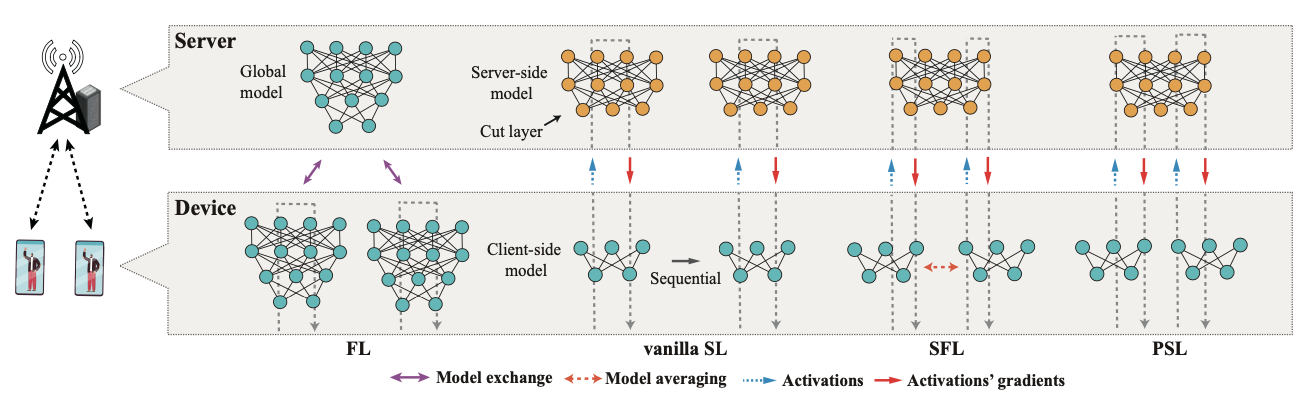
\includegraphics[scale=0.65]{figures/split-learning.png}
	\caption{An example of the structure of a network implementing SL for model trainig
		\cite{split-learning}}
\end{figure}
SL is just a piece of the intricate puzzle that we need to build, it allows us to have fast training
procedures, supposing the model has been devided effectively, but it forces us to have the model
fragmented in different parts of the network and this complicates things because we want the model
to be "local" to the user, or at least the part that has been fine-tuned for his use.
To grant this locality property we will need to have load balancing algorithms or RLMs that can
handle the choice of model migration.

Although SL makes the training process possible while keeping user's private data safe, it
introduces complications on the inference side, depending on the number of sections that the model
has been partitioned into the inference process is going to require the participation of all the
computing elements that store a part of the whole model. This implies a discrete volume of data that
needs to be moved between the various compute elements in order to allow the calculation of the
results.

Since the process leads to a very clear network strain we will be seeing in the following a series
of compression techniquest that allow the reduction of the amount of data that need to be moved in
the network to complete the inference process.

\bigskip
\noindent
LOW-RANK ADAPTATION

LOw-Rank Adaptation (LoRA) is a technique that freezes the pretrained model weights and injects
trainable rank decomposition matrices into each layer of the Transformer architecture, greatly
reducing the number of training parameters for downstream tasks.

This technique really strikes the point because it's of the utmost importance to be able to reduce
the number of trainable parameters for the constrained models that will need to face some sort of
fine-tuning procedure in the END. Instead of doing a fine-tuning of the complete model we just take
a look at Figure \ref{fig:lora}.
\begin{figure}
	\phantomcaption
	\label{fig:lora}
	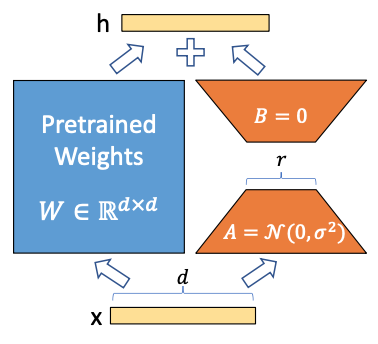
\includegraphics{figures/lora.png}
	\caption{The LoRA approach proposed in \cite{}}
\end{figure}
Per the studies made in article \cite{}, given a weight matrix $W_0 \in \R^{d \times k}$ we can
actually represent it via a low-rank decomposition like:
\begin{equation}
	W_0 + \Delta W = W_0 + B \cdot A
\end{equation}
where $B \in \R^{d \times r}, A \in \R^{r \times k}$ and the rank $r$ is much smaller than either
$d$ (which is the full rank of the dense layers' decomposition matrices, in the case of GPT-3 the
count can get up to 12.288, which makes them really huge matrices) or $k$, and these are the ones
shown in \ref{fig:lora}. The result is an extremely underdimensioned matrix with respect to the ones that we would have had to work with in origin.

The gradient updates for the matrix $W_0$ are frozen while $A$ and $B$ contain the trainable
parameters.

When utilizing this technique in the field of Transformers (which is fundamental inside LLM
architectures) the empirical results when using GPT-3 175B were the following:
\begin{itemize}
	\item slicing VRAM of up to $2/3$ since there is no need to store Adam optimizer states for
		the frozen parameters (they went from 1.2 TB to 350GB of VRAM usage).
	\item If the rank of the decomposition was 4 and, of all the transformer matrices, only the
		value projection and query matrices were adapted the checkpoint size is reduced of
		circa 10000 times which in turns means very easy model switching due to the
		forgettable size of LoRA weights.
\end{itemize}
To provide another reason for LoRA, it's really easy to implement next to other techniques. I would
go as far as to say that it's essential to allow the correct implementation of distributed
learning techniques like SL because even the partial retrain of a network for fine-tuning might be
too expensive for the underpowered nodes at the END of the 6G network.

\clearpage


\noindent
\textbf{FUTURE CHALLENGES:}
\phantomsection
\makeatletter\def\@currentlabel{\texttt{(IV)}}\makeatother
\label{sec:future-challenges}
\\
\externaldocument{../main.tex}
Everything that has been introduced to this point has that \textit{je ne sais quoi} of feasible, we
have all of the pieces needed to build the puzzle and the direction seems to be the right one, all
that is required now is just research to see how the various components interact and if there is
anything that can be done to increase the performance, or the efficiency.

As with any other progress in the field of computer science, but more so with this one than any
other, having the guarantee of dealing with an extremely efficient system that can do inference and
train complex models with by making compromises with the lowest possible overhead might reduce
dramatically the amount of ENs that would need to be deployed at the edge of the various cells
introduced in \ref{sec:opportunities} (ENs are very costly to produce because necessitate the help of GPUs to perform
training and inference efficiently).

Many important steps forward have been made when it comes to LLM optimization and we achieved very
good results even when deployed in resource constrained conditions, this does not mean, though, that
the research is over. While with a model like QLoRA it's possible to fine-tune a 65B model in just
under 24 hours with a single GPU there is going to be the need of fine-tuning and training more than
just one model at the same time, in the meanwhile the ENs and END devices
will have to cooperate to do inference and solve more classical requests that do not necessarily require AI
intervention.

That is why it's still necessary to put a lot of work in the field of inference and training
optimization at low precisions using instruments like LoRA, QLoRA and quantization; furthermore, as
was shown in \ref{sec:technical-limitations} SL is a very powerful technique that makes training possible even in constrained
environments (especially if paired with quantization techniques), more work should be put in trying
to solve the problem of finding optimal splitting points for models using RLMs or other heuristic
techniques based on different network parameters (as was shown in \cite{rlm-split-learning}).

Last but not least, there is no framework that puts all of the ingredients together, therefore it's
of the maximum importance to start working in that direction to solve the orchestration problems
that arise from working with an architecture as complex as 6G's. Some questions that could be
interesting for future research could be the following:
\begin{itemize}
	\item How to handle the mobility of users and how to guarantee the principle of locality of
	      the model shards generated via SL?
	\item How to efficiently split the network in order to maintain good inference performance
	\item How to handle model caching
\end{itemize}


\clearpage
\printbibliography
\end{document}
